\newpage
\section{Entwurfsphase}
\label{sec:Entwurfsphase}

\subsection{Architekturdesign}
\label{sec:Architekturdesign}
\begin{wrapfigure}{r}{0.5\textwidth} % r = rechts, Breite = 50% der Textbreite
    \centering
    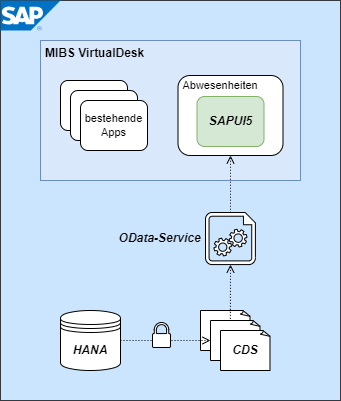
\includegraphics[width=\linewidth, keepaspectratio]{Bilder/Komponenten.png} % Bild einfügen
    \caption{Komponenten}
    \label{fig:Komponenten}
\end{wrapfigure}

Das Architekturdesign der Anwendung basiert auf einer modularen Struktur, bei der verschiedene Komponenten zusammenarbeiten. Dies soll die Wiederverwendbarkeit und Wartbarkeit der einzelnen Komponenten erhöhen. 
Die Anwendung wird als SAP Fiori App innerhalb des MIBS VirtualDesk, welches auf einem SAP Fiori Launchpad basiert, veröffentlicht. Das Frontend wird, mithilfe des SAP Fiori Frameworks, als „Fiori Freestyle“-App\footnote{Entwicklungsansatz für individuell entwickelte SAP Fiori-Anwendung ohne Vorlagen} implementiert. Dieses erfordert einen höheren Entwicklungsaufwand, bietet dafür jedoch eine bessere Erweiterbarkeit der Benutzeroberfläche.

Der OData-Service\footnote{Open Data Protocol - standardisiertes Protokoll für Zugriff auf Daten über das Web} stellt das zentrale Bindeglied zwischen dem Frontend und der Datenquelle dar. Er ermöglicht den selektiven Zugriff auf die relevanten Abwesenheitsdaten der Mitarbeiter. Die Daten, die durch diesen Service abgerufen werden, basieren auf Core Data Services (CDS) Views, die in SAP S/4HANA definiert sind. Diese CDS Views werden mit dem SAP-Berechtigungssystem verknüpft, sodass nur autorisierte Benutzer Zugriff auf die entsprechenden Informationen haben.

%-	Entwickung + Tests auf dev system?

Insgesamt ermöglicht dieses Design eine sichere, performante und benutzerfreundliche Darstellung der Abwesenheitsinformationen, die in Echtzeit im Fiori Launchpad bereitgestellt werden. Das Zusammenspiel aus SAPUI5-Frontend, OData-Service und CDS Views stellt sicher, dass die Anwendung sowohl flexibel als auch an die speziellen Anforderungen der MIBS AG angepasst ist.

\subsection{UI Design}
\label{sec:UI Design}
Das User Interface (UI) wird mit Hilfe des SAP Fiori Frameworks so gestaltet, dass es eine intuitive Kalenderübersicht der Mitarbeiter-Abwesenheiten der MIBS bietet. Der Kalender wird den zentralen Bestandteil der Oberfläche bilden und die Abwesenheiten aller Mitarbeiter als Termine darstellen. Verschiedene Abwesenheitstypen (\zB Krankheit, Urlaub, Sondertage) werden durch unterschiedliche Farben und Symbole gekennzeichnet, um diese somit auf einen Blick erkenntlich zu machen. Jeder Kalendereintrag wird Informationen wie Start- und Enddatum sowie den Abwesenheitsstatus enthalten.
Filter- und Suchfunktionen werden eine gezielte Auswahl bestimmter Mitarbeiter ermöglichen. Die Navigation wird durch Dropdown-Menüs und Eingabefelder unterstützt, um eine schnelle Bedienung innerhalb der App zu gewährleisten.
Eine grafischer Entwurf befindet sich im \Anhang{app:UI-Design}.

\subsection{Serverseitige Logik}
\label{sec:Serverseitige Logik}
Die serverseitige Logik wird aus CDS Views bestehen, die als Datenquelle fungieren. Auf diesen Views soll ein OData-Service aufgesetzt werden, welcher als Web API erreichbar sein soll. Hierbei werden keine Daten verändert, sondern nur abgerufen und im OData-Format an die Clients zur Verfügung gestellt. Die Kommunikation erfolgt dabei über HTTPS. Die CDS Views sollen den Zugriff auf die benötigten Daten sicherstellen, indem sie die Daten aus den bestehenden Tabellen filtern sowie formatieren.

\subsubsection{Datenbasis}
\label{sec:Datenbasis}

Wie bereits in der \Anhang{app:Datenanalyse} aufgelistet, müssen Einträge aus diversen Tabellen kombiniert werden. Um alle benötigten Daten, wie im \Anhang{app:Lastenheft} unter \hyperref[Abwesenheitsarten]{3.2 Abwesenheitsarten} gewünscht, zusammen zu führen, müssen für jedem Mitarbeiter deren Krankheitstage, Urlaubstage sowie besondere Tage, zu welchen unter anderem die Schulzeiten der Auszubildenden zählen, selektiert werden. Die Views sollen, wie im \Anhang{app:CDS Views} beschrieben, angelegt werden.
Da die Abwesenheiten in verschiedenen Tabellen gespeichert sind, werden diese mit einem \Code{UNION-SELECT} vereinigt.
% Tabellen auflisten aus denen selektiert wird?

\subsubsection{Islands and Gaps Problem}
\label{sec:Islands and Gaps Problem}

Das „Islands and Gaps“-Problem beschreibt eine Situation, bei der man in einer Datenreihe zusammenhängende Bereiche („Islands“) und Lücken dazwischen („Gaps“) identifizieren möchte. 

Anders als beispielsweise die Schulblöcke, werden die Urlaubstage für jeden Tag einzeln abgespeichert, da diese verschiedene Eigenschaften haben können, wie etwa Halbtagesurlaub oder Sonderurlaub. Befindet sich ein Mitarbeiter eine Woche lang im Urlaub, werden im System fünf separate Einträge angelegt. Im User Interface soll jedoch ein zusammenhängender Urlaubsblock als ein einziger Termin dargestellt werden. Diese Anforderung lässt sich auf das Islands and Gaps-Problem übertragen.

Die Lösung erfolgt in zwei Selektionsschritten. Zunächst werden die „Islands“ identifiziert, indem der Index der Datensätze mit dem Datum verglichen wird. Da der Index und das Datum bei aufeinanderfolgenden Tagen im gleichen Intervall iterieren, können zusammenhängende Krankheitstage als abstrakte Gruppen zusammengefasst werden. \TabelleRef{tab:Island and Gaps Beispiel} veranschaulicht einen exemplarischen Ablauf dieses Verfahrens.

%\begin{wraptable}{r}{0.5\textwidth}
\tabelle{Island and Gaps Beispiel}{tab:Island and Gaps Beispiel}{Island and Gaps Beispiel}
%\end{wraptable}

Anschließend wird mit einer weiteren Selektion, die nach diesen Gruppen aggregiert, das Anfangs- und Enddatum ermittelt. Dazu werden die Aggregatfunktionen \Code{MIN} und \Code{MAX} verwendet, um für jede Gruppe den frühesten sowie spätesten Krankheitstag festzulegen um so die Krankheitsperiode als zusammenhängenden Zeitraum abzubilden.

\subsubsection{Zugriffskontrolle}
\label{sec:Zugriffskontrolle}
Die Zugriffskontrolle auf die CDS Views wird durch die Rechteverwaltung im SAP-System gewährleistet. Dabei werden die Berechtigungen für die Benutzer anhand der bestehenden Rollen und Berechtigungsobjekte gesteuert. Auf die CDS Views wird eine Berechtigungsprüfung angewendet, die es sowohl dem Vorstand als auch dem Backoffice ermöglicht, die Daten aller Mitarbeiter einzusehen. Teamleiter hingegen erhalten nur Zugriff auf die Mitglieder ihres eigenen Teams.

\subsubsection{OData-Service}
\label{sec:OData-Service}
Da die Bereitstellung der Daten über einen OData-Service erfolgen soll, musste zunächst eine Entscheidung zur Implementierungsmethode getroffen werden. Hier standen die Technologien \textbf{SEGW} und \textbf{SADL} zur Auswahl, die beide die Veröffentlichung eines OData-Service direkt aus einem SAP-System ermöglichen. Zusätzlich war die Wahl der passenden \textbf{OData-Service-Version} erforderlich.

Zur fundierten Entscheidungsfindung wurde eine Nutzwertanalyse durchgeführt, angefügt im \Anhang{app:Nutzwertanalyse}. Dafür wurden zunächst die wichtigsten Kriterien ermittelt und mit individuellen Gewichtungen versehen. Im Anschluss wurden die vier möglichen Optionen in Bezug auf jedes Kriterium bewertet, wobei die Ergebnisse mit den festgelegten Gewichtungen multipliziert wurden. Die Option mit der höchsten Gesamtpunktzahl wurde als die beste Wahl identifiziert.


\subsection{Testkonzept}
\label{sec:Testkonzept}
Zur Sicherstellung der Anwendungsintegrität wurde im Vorfeld der Umsetzung eine umfassende Testmatrix entwickelt. Diese Matrix umfasst eine Vielzahl von \textbf{Whitebox-} und \textbf{Blackbox-Tests} sowie die Vorgabe der Nutzung weiterer Tools zum Testen der Anwendung. Diese sollen sowohl funktionale als auch sicherheitsrelevante Aspekte der Anwendung abdecken und eine hohe Zuverlässigkeit gewährleisten. Ein Ausschnitt der Testmatrix befindet im \Anhang{app:Testmatrix}.

\subsection{Pflichtenheft}
\label{sec:Pflichtenheft}
Zum Schluss der Entwurfsphase wurde das Pflichtenheft erstellt. Aufbauend auf dem \Anhang{app:Lastenheft} beschreibt dieses die gewünschten Anforderungen. Es dient als Leitfaden für die Realisierung des Projektes. Ein Auszug des Pflichtenheft befindet sich im \Anhang{app:Pflichtenheft}.